\documentclass{report}
\usepackage[MeX]{polski}
\usepackage[utf8]{inputenc}
\usepackage[T1]{fontenc}

\usepackage{amsfonts}
\usepackage{amsthm}
\usepackage{amsmath}
\usepackage{amssymb}
\usepackage{float}
\usepackage{enumerate}
\usepackage{fancyhdr}
\usepackage{latexsym}
\usepackage{wasysym}
\usepackage{graphicx}
\usepackage[hmarginratio=1:1]{geometry}
\graphicspath{{plots/}}

\addtolength{\voffset}{-1cm}
\addtolength{\textheight}{+2cm}
\addtolength{\hoffset}{-1cm}
\addtolength{\textwidth}{+2cm}

\newcommand{\bc}{\begin{cases}}
\newcommand{\ec}{\end{cases}}
\newcommand{\cc}{^{\circ}}
\newcommand{\sq}{\begin{flushright}$\square$\end{flushright}}
\renewcommand\Re{\operatorname{\mathfrak{Re}}}
\renewcommand\Im{\operatorname{\mathfrak{Im}}}
\newcommand{\imp}{\Rightarrow}
\newcommand{\pair}[1]{\langle #1 \rangle}
\renewcommand{\epsilon}{\varepsilon}
\newcommand{\eps}{\epsilon}
\newcommand{\I}{\imath}
\newcommand{\fl}[1]{\left\lfloor #1 \right\rfloor}
\newcommand{\ceil}[1]{\left\lceil #1 \right\rceil}
\newcommand{\clim}{\lim_{n \to \infty}}
\newcommand{\csum}{\sum_{n=1}^{\infty}}
\newcommand{\Zp}[1]{\mathbb{Z}_{#1}}
\newcommand{\Zi}{\mathbb{Z}[\I]}
\newcommand{\Ze}{\mathbb{Z}[\omega]}
\newcommand{\RR}{[-\infty; +\infty]}
\newcommand{\lin}{\mathrm{lin}}
\newcommand{\sgn}{\mathrm{sgn}}
\newcommand{\tr}{\mathrm{tr}}
\newcommand{\grad}{\mathrm{grad}}
\newcommand{\vol}{\mathrm{vol\,}}
\newcommand{\graph}{\mathrm{graph}}
\newcommand{\R}{\mathbb{R}}
\newcommand{\N}{\mathbb{N}}
\newcommand{\Z}{\mathbb{Z}}
\newcommand{\C}{\mathbb{C}}
\renewcommand{\P}{\mathbb{P}}
\newcommand{\Mst}[1]{M(#1)^{\mathrm{st}}_{\mathrm{st}}}
\newcommand{\st}{\mathrm{st}}
\newcommand{\ppp}[2]{\frac{\partial #1}{\partial #2}}
\newcommand{\pis}[1]{\mathcal{#1}}
\newcommand{\set}[1]{\{#1\}}
\renewcommand{\phi}{\varphi}
%\newcommand{\norm}[1]{\left|\left|#1\right|\right|}
\newcommand{\norm}[1]{N(#1)}
\newcommand{\abs}[1]{\left|#1\right|}

\def\thesection {\arabic{section}.}
\def\thesubsection {\alph{subsection})}
\def\thesubsubsection {\arabic{subsubsection}.}

\makeatletter
\renewcommand*\env@matrix[1][*\c@MaxMatrixCols c]{
 \hskip -\arraycolsep
 \let\@ifnextchar\new@ifnextchar
 \array{#1}}
\makeatother

\newcommand{\muz}[1]{\mu^{*}\left(#1\right)}
\newcommand{\leb}[1]{\lambda^{*}\left(#1\right)}
\newcommand{\cnt}{\mathrm{count}}

\renewcommand{\d}{\partial}

\title{Obliczeniowe badanie oczekiwanego zachowania \\ dzielników pierwszych \\ liczb naturalnych}
\author{Maciej Dębski}

\begin{document}

\maketitle

\chapter*{Podstawy teoretyczne}
Jak wiadomo z podstaw teorii liczb, każdą liczbę naturalną $n \in \N$ można przedstawić jako
$$ n = p_1 \cdot p_2 \cdot p_3 \cdot \ldots \cdot p_k, \quad p_i \in \P. $$
Będziemy tutaj rozpatrywać podobne przedstawienie, tylko uporządkowane według rozmiaru $p_i$ i uzupełnione jedynkami do stałej długości $K$:
$$ n = a_1 \cdot a_2 \cdot \ldots \cdot a_K, \quad a_i \in \P \cup \set{1}, a_1 \geq a_2 \geq \ldots \geq a_K. $$
Takie przedstawienie zawsze istnieje dla odpowiednio dużego $K$, np. dla $K > \log_2(n)$. \\

Będę badał średni rozmiar dzielników $a_i$ w porównaniu z $n$. W szczególności ciekawe wyniki daje badanie ich logarytmów o podstawie n. Możemy zapisać
$$ n = n^{\gamma_1} \cdot \ldots n^{\gamma_K}, \quad \gamma_i = \log_n{a_i}. $$
Oczywiście, po zlogarytmowaniu stronami otrzymujemy
\begin{equation} \label{sum} 1 = \gamma_1 + \ldots + \gamma_K. \end{equation} \\

Zdefiniujmy teraz badane średnie. Niech $\gamma_i(n), i \in \set{1, \ldots, K}$ oznacza odpowiednią wartość z rozkładu $n$, jak powyżej. Dla ustalonego $N$, przyjmijmy
$$ \bar{\gamma}_i = \frac{1}{N} \sum_{n=1}^{N} \gamma_i(n). $$
Obliczenia wskazują, że dla każdego $i$, ciąg $\bar{\gamma}_i$ jest zbieżny dla $N \to \infty$. Ponadto, suma tych ciągów wydaje się szybko zbiegać do $1$,
co jest odpowiednikiem równości (\ref{sum}) dla średnych.

\chapter*{Metoda obliczeń}

Obliczenia przeprowadziłem dla $N = 10^9$ i $K = 30$, na pojedynczym komputerze z procesorem i7-3537U (2.00GHz) i 10GB pamięci RAM.
Program napisałem w C++, a następnie mocno zoptymalizowałem i sprofilowałem - początkowe wersje działały kilka rzędów wielkości wolniej.
Ostateczne obliczenia trwały poniżej 10 minut. Kod programu oraz dane wynikowe jest dostępny w repozytorium projektu: https://github.com/mdebski/atl

\section*{Algorytm}
Jednym z głównych problemów przy pisaniu programu było kontrolowanie zużycia pamięci. Tablica liczb (uint32\_t) wielkości $N = 10^9$ zajmuje $4GB$ pamięci, i dwie takie tablice już się nie mieściły, przy standardowym zużyciu pamięci przez system.
Stąd na przykład niemożliwe było zapisanie pełnego rozkładu na czynniki pierwsze wszystkich rozpatrywanych liczb. \\

Problem podzieliłem na dwie części. W pierwszej za pomocą sita znajdowałem pewien dzielnik pierwszy dla każdej z liczb. Sprytna implementacja sita pozwoliła
na osiągnięcie gwarancji że jest to najmniejszy dzielnik pierwszy, bez ograniczania prędkości sita. Następnie łatwo obliczyć największy dzielnik pierwszy - przechodząc dynamicznie tablicę od najmniejszych liczb, możemy obliczyć:
$$ MaxPrimeDivisor[n] = max(MinPrimeDivisor[n], MaxPrimeDivisor[n/MinPrimeDivisor[n]]). $$

W następnym etapie korzystając z obliczonej tablicy największych dzielników obliczałem $\bar{\gamma}_1, \ldots \bar{\gamma}_K$. Warto zauważyć, że wszystkie dzielniki pierwsze $n$, wraz z krotnościami, uporządkowane od największego, to:
$$ p_1 = MaxPrimeDivisor[n] $$
$$ p_2 = MaxPrimeDivisor[n/p_1] $$
$$ p_3 = MaxPrimeDivisor[n/p_2] $$
$$ \ldots $$
W ten sposób dla każdej liczby obliczałem wszystkie dzielniki i odpowiednie wyrażenia $\log(p_i)/\log(n)$ i dodawałem je do akumulatorów.

\section*{Optymalizacje}

W pierwszej części zoptymalizowałem zużycie pamięci rezygnując z pamiętania całej tabeli dla sita - zamiast tego, trzymałem tylko dzielniki dla liczb względnie pierwszych z $15 = gcd(2, 3, 5)$,
a dla pozostałych obliczałem je na bieżąco - dzieląc przez $2, 3, 5$. Pozwoliło to na zużycie $15 / phi(15) \simeq 4$ razy mniej pamięci. Dla przyspieszenia poprzez zwiększenie lokalności odwołań do pamięci
użyłem sita segmentowanego, według http://primesieve.org/segmented\_sieve.html. \\

W drugiej części istotną część kosztu stanowiło obliczanie logarytmów. Z tego powodu wpierw stablicowałem wartości logarytmów liczb pierwszych mniejszych od $10^9$.
Jako że jest ich tylko około $5\cdot 10^7$ nie stanowiło to dużego narzutu pamięciowego. Do ich przechowywania istotnie lepiej zadziałała mapa boost::container::flat\_map niż std::map.
Ponadto, zmodyfikowałem wewnętrzną pętle by nie obliczała $\log(n)$ dla każdego $p_i$, a tylko jednokrotnie. Oczekiwałem że kompilator sam to zrobi w ramach optymalizacji wspólnych podwyrażeń, ale się przeliczyłem.

\chapter*{Wyniki}

\section*{Szacowanie $\bar{\gamma_i}$}

\begin{center} 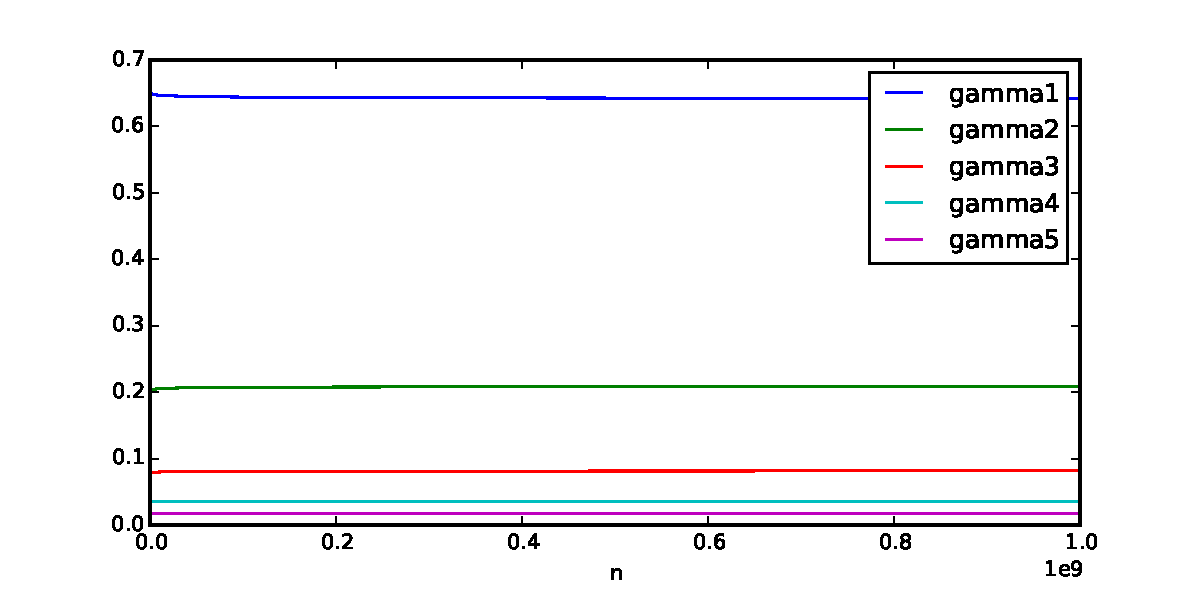
\includegraphics[width=0.75 \linewidth]{0} \end{center}
\begin{center} 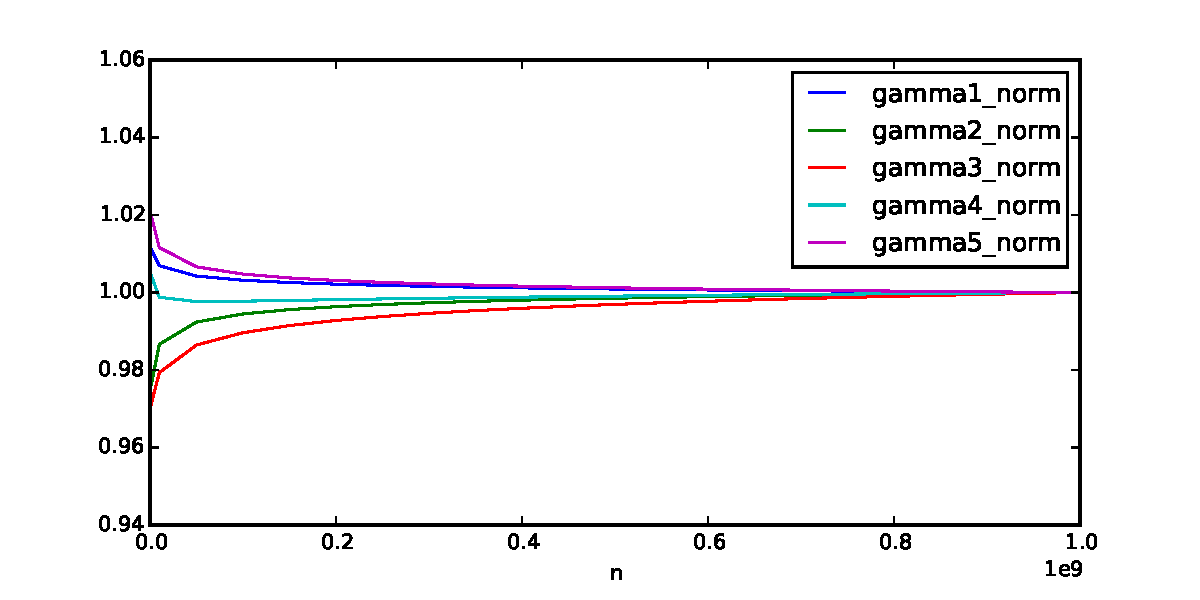
\includegraphics[width=0.75 \linewidth]{1} \end{center}

\section*{Zależności pomiędzy $\bar{\gamma_i}$}

\begin{center} 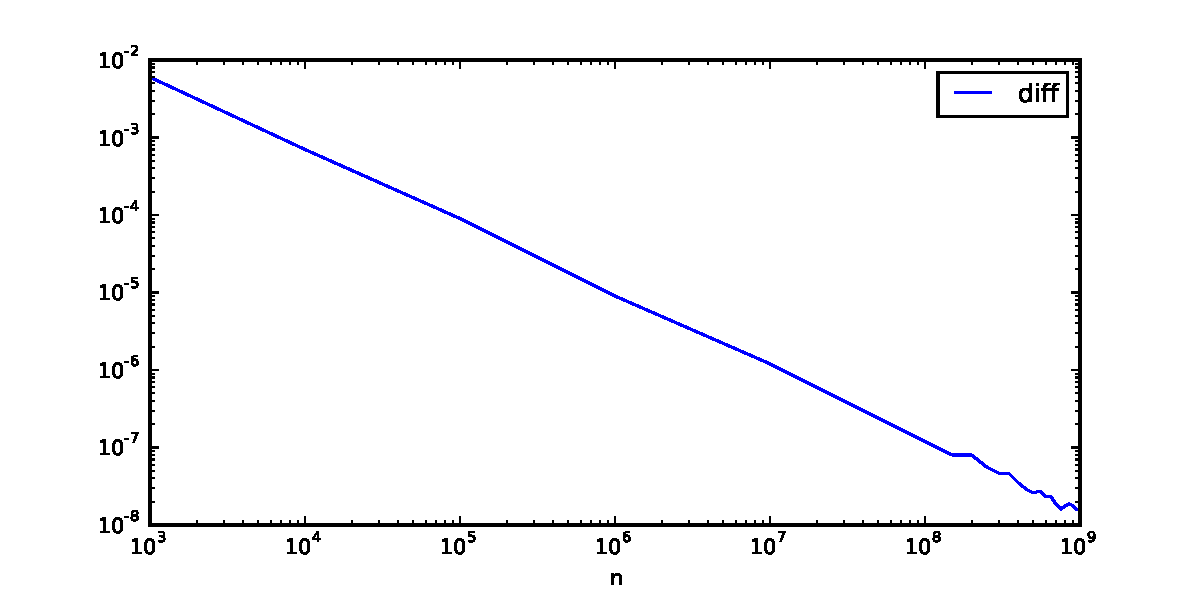
\includegraphics[width=0.75 \linewidth]{2} \end{center}
\begin{center} 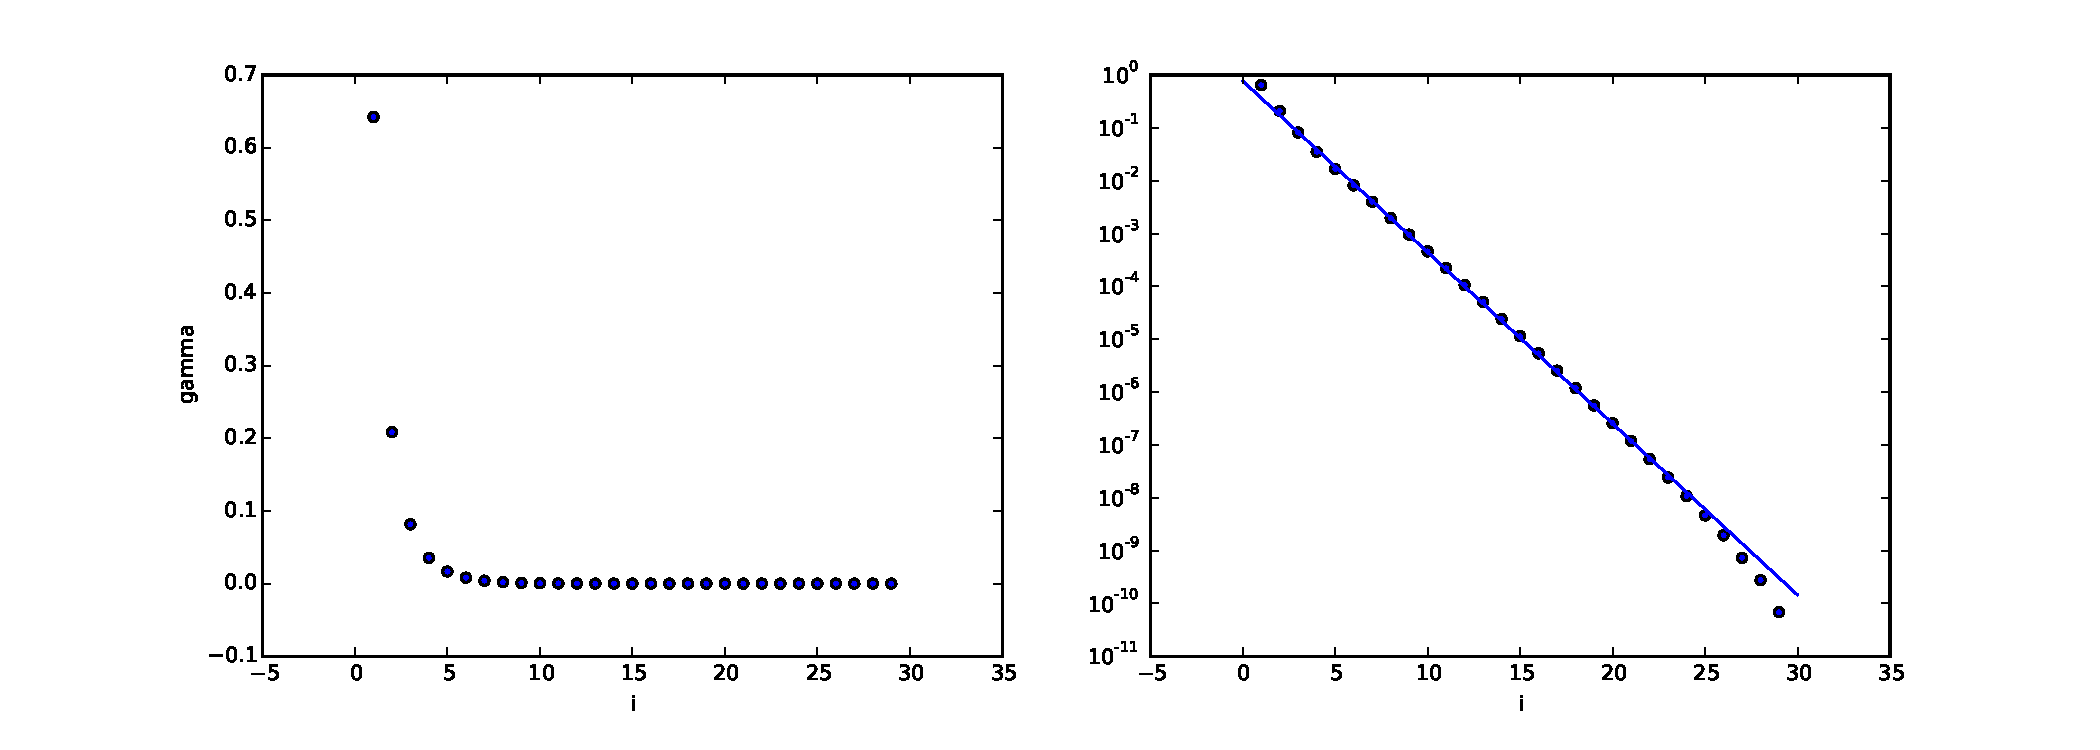
\includegraphics[width=1 \linewidth]{3} \end{center}

\end{document}
